\section{Intuición Geométrica y Notación Matricial}

Un sistema de ecuaciones lineales puede interpretarse geométricamente como un conjunto de planos (en \(\mathbb{R}^3\)) o, en general, hiperplanos (en \(\mathbb{R}^n\)). Resolver el sistema equivale a encontrar el punto —o conjunto de puntos— donde todos estos objetos geométricos se intersecan simultáneamente.

Según la configuración relativa, pueden darse tres situaciones fundamentales (ver Figura \ref{fig:tipos_soluciones}):

\begin{itemize}
    \item \textit{Solución única:} Los planos se intersecan en un único punto (sistema compatible determinado).
    \item \textit{Infinitas soluciones:} Los planos comparten una recta o un eje común, como las páginas de un libro abierto (sistema compatible indeterminado).
    \item \textit{Sin solución:} No existe un punto común a todos; por ejemplo, planos paralelos como los pisos de un edificio o formando un prisma triangular (sistema incompatible).
\end{itemize}

En la figura \ref{fig:planos_3d} se ilustra la interpretación en 3D, donde cada ecuación representa un plano en el espacio tridimensional. La solución del sistema corresponde al punto (o conjunto de puntos) donde estos planos se intersectan. Si la solución es única, los planos se cruzan en un solo punto; si hay infinitas soluciones, los planos se intersectan a lo largo de una línea o plano común; y si no hay solución, los planos no se intersectan en absoluto.

\begin{figure}[h]
    \centering
    \begin{minipage}{0.48\textwidth}
        \centering
        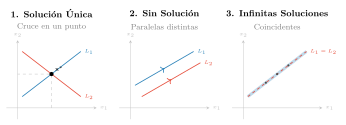
\includegraphics[width=0.8\textwidth]{images/sistemas_soluciones.pdf}
        \caption{Casos en 2D (Rectas).}
        \label{fig:tipos_soluciones}
    \end{minipage}
    \hfill
    \begin{minipage}{0.48\textwidth}
        \centering
        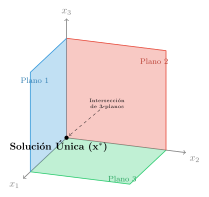
\includegraphics[width=0.8\textwidth]{images/interpretacion_3d.pdf}
        \caption{Intersección en 3D (Planos).}
        \label{fig:planos_3d}
    \end{minipage}
\end{figure}

\subsubsection*{El concepto de Hiperplano y la Ceguera Dimensional}
Mientras que en 2D visualizamos rectas y en 3D planos, los problemas reales en agroambiental (como datos satelitales con 12 bandas espectrales) o mecatrónica (un robot con 7 grados de libertad) habitan en espacios de dimensión superior.

Aquí surge el concepto de \textbf{hiperplano}: una generalización matemática que representa un subespacio ``plano'' de dimensión \(n-1\) en un espacio de dimensión \(n\). Aunque nuestra intuición biológica está limitada a tres dimensiones, el álgebra lineal no sufre esta restricción. La ecuación:
\[ 2x_1 + 5x_2 - x_3 + 8x_4 = 10 \]
describe un hiperplano en \(\mathbb{R}^4\). No podemos dibujarlo, pero podemos operar con él algebraicamente con la misma facilidad que con una recta. El álgebra se convierte así en nuestros ``ojos'' que nos permite ver y manipular estructuras en dimensiones que nuestro cerebro no puede concebir.


\subsection{1. Eliminación Gaussiana (El Algoritmo Paso a Paso)}

Este es el algoritmo fundamental. Su objetivo es transformar un problema complejo (sistema acoplado) en uno sencillo (sistema triangular) mediante operaciones que no alteran la solución.

El proceso tiene dos fases:
\begin{enumerate}
    \item \textbf{Eliminación hacia adelante:} Convertir la matriz original $A$ en una matriz triangular superior $U$ (hacer ceros debajo de la diagonal).
    \item \textbf{Sustitución hacia atrás:} Despejar las incógnitas empezando por la última ecuación.
\end{enumerate}

\subsubsection*{Ejemplo Práctico 3x3}
Consideremos el siguiente sistema. Para manipularlo numéricamente, formamos la \textbf{matriz aumentada} $[A|\mathbf{b}]$, que incluye los términos independientes:

\[
\begin{cases}
2x_1 + \phantom{1}x_2 + \phantom{1}x_3 = 4 \\
4x_1 - 6x_2 \phantom{+ 0x_3} = -2 \\
-2x_1 + 7x_2 + 2x_3 = 7
\end{cases}
\implies
\left[
\begin{array}{ccc|c}
\mathbf{2} & 1 & 1 & 4 \\
4 & -6 & 0 & -2 \\
-2 & 7 & 2 & 7
\end{array}
\right]
\]

\textbf{Paso 1: Primer Pivote (Columna 1)} \\
Nuestro objetivo es eliminar los números debajo del primer elemento de la diagonal (el \textbf{2}, llamado pivote).
\begin{itemize}
    \item Para eliminar el $4$ (Fila 2): Hacemos $F_2 \leftarrow F_2 - 2F_1$.
    \item Para eliminar el $-2$ (Fila 3): Hacemos $F_3 \leftarrow F_3 + F_1$.
\end{itemize}

\[
\left[
\begin{array}{ccc|c}
2 & 1 & 1 & 4 \\
\mathbf{0} & -8 & -2 & -10 \\
\mathbf{0} & 8 & 3 & 11
\end{array}
\right]
\]

\textbf{Paso 2: Segundo Pivote (Columna 2)} \\
Ahora nos enfocamos en la sub-matriz restante. El nuevo pivote es el $-8$. Necesitamos eliminar el $8$ que está debajo de él.
\begin{itemize}
    \item Operación: $F_3 \leftarrow F_3 + F_2$.
\end{itemize}

\[
\left[
\begin{array}{ccc|c}
2 & 1 & 1 & 4 \\
0 & -8 & -2 & -10 \\
0 & \mathbf{0} & 1 & 1
\end{array}
\right]
\]

¡El sistema ya está triangulado! Observa que hemos obtenido ceros en el "triángulo" inferior izquierdo.

\textbf{Paso 3: Sustitución hacia atrás} \\
Reescribimos el sistema equivalente que nos ha quedado, que ahora es trivial de resolver de abajo hacia arriba:

1. \textbf{Tercera ecuación:}
   \[ 1x_3 = 1 \implies \mathbf{x_3 = 1} \]

2. \textbf{Segunda ecuación} (sustituyendo $x_3$):
   \[ -8x_2 - 2(1) = -10 \implies -8x_2 = -8 \implies \mathbf{x_2 = 1} \]

3. \textbf{Primera ecuación} (sustituyendo $x_2, x_3$):
   \[ 2x_1 + 1 + 1 = 4 \implies 2x_1 = 2 \implies \mathbf{x_1 = 1} \]

La solución del sistema es el vector $\mathbf{x} = [1, 1, 1]^\top$. Computacionalmente, este proceso tiene una complejidad de $O(n^3)$, lo que significa que si duplicamos el número de variables, el tiempo de cálculo se multiplica aproximadamente por 8.
\begin{appbox}{Aplicación: Balanceo de Cargas en Drones}
En el diseño del chasis de un dron fumigador, las fuerzas estáticas se resuelven mediante Gauss. Como la estructura del dron no cambia, el método es directo y exacto para asegurar que los brazos soporten el tanque de líquido.
\end{appbox}

\subsection{2. Método de la Matriz Inversa}
Teóricamente, si $A$ es cuadrada y su determinante es no nulo ($\det(A) \neq 0$), existe una matriz $A^{-1}$ tal que:

$$ \mathbf{x} = A^{-1}\mathbf{b} $$

Aunque matemáticamente elegante, computacionalmente es costoso. Calcular la inversa requiere muchas más operaciones que la eliminación gaussiana.

\begin{alertblock}{Advertencia Computacional}
En sistemas grandes (ej. análisis de genoma vegetal o simulación de fluidos), **nunca** se calcula la inversa explícita. Es numéricamente inestable y lenta. Se prefieren métodos de descomposición.
\end{alertblock}

\subsection{3. Descomposición LU (Lower-Upper)}
Este es el método "rey" en la ingeniería aplicada. Consiste en factorizar la matriz $A$ en el producto de dos matrices triangulares: una inferior ($L$) y una superior ($U$).
$$ A = L \cdot U $$
Esto permite resolver el sistema en dos pasos rápidos y baratos computacionalmente. Es ideal cuando tenemos una misma matriz $A$ (ej. un robot) pero múltiples vectores $\mathbf{b}$ (diferentes posiciones objetivo).

\section{Conexión Agro-Mecatrónica: Sensores Espectrales}

\begin{agrobox}{Calibración de Sensores Multiespectrales}
Imagina un sensor que mide la salud de una planta. El sensor tiene 3 fotodiodos, pero cada uno tiene una ligera "contaminación" de otras longitudes de onda (crosstalk).
\begin{itemize}
    \item Lectura Diodo Rojo = $1.0 \cdot \text{RojoReal} + 0.1 \cdot \text{VerdeReal}$
    \item Lectura Diodo Verde = $0.2 \cdot \text{RojoReal} + 0.9 \cdot \text{VerdeReal}$
\end{itemize}
Para recuperar los valores reales de luz (RojoReal, VerdeReal) a partir de las lecturas sucias del sensor, debemos resolver el sistema usando la matriz de calibración inversa del fabricante.
\end{agrobox}

\section{Implementación en Python (NumPy)}

A diferencia del capítulo anterior donde usamos optimización (TensorFlow), aquí usaremos álgebra lineal exacta con **NumPy**, la librería base de la ciencia de datos.

\begin{lstlisting}[language=Python, caption={Resolución exacta de sistemas lineales con NumPy}]
import numpy as np

# 1. Definir el sistema (Ejemplo de calibración de sensores)
# Matriz de coeficientes (Crosstalk del sensor)
A = np.array([
    [1.0, 0.1, 0.05], # Diodo 1 sensible a Banda 1, 2 y 3
    [0.2, 0.9, 0.1],  # Diodo 2
    [0.1, 0.2, 0.8]   # Diodo 3
])

# Vector b (Lecturas crudas del sensor)
b = np.array([500, 800, 300]) # Valores en milivoltios

# 2. Método 1: Resolución directa (Usa LU internamente - RECOMENDADO)
# Es el metodo mas rapido y estable numéricamente
x_solve = np.linalg.solve(A, b)

# 3. Método 2: Calculando la Inversa explícita (NO RECOMENDADO para N grande)
A_inv = np.linalg.inv(A)
x_inv = np.dot(A_inv, b)

# 4. Verificación
print("--- Resultados de Calibración ---")
print(f"Valores reales de luz: {x_solve}")

# Comprobamos si Ax = b
check = np.dot(A, x_solve)
print(f"Reconstrucción de lecturas (Check): {check}")
print(f"Error numérico: {np.allclose(check, b)}")
\end{lstlisting}

%\begin{figure}[h]
%    \centering
%    \includegraphics[width=0.8\textwidth]{images/planos_interseccion}
%    \caption{Representación visual de la solución única como intersección de planos en $\mathbb{R}^3$.}
%    \label{fig:planos}
%\end{figure}